\documentclass[10pt, letterpaper, conference]{IEEEtran}
% a4paper
% Add the compsocconf option for Computer Society conferences.
%
% If IEEEtran.cls has not been installed into the LaTeX system files,
% manually specify the path to it like:
% \documentclass[conference]{../sty/IEEEtran}


% *** CITATION PACKAGES ***
%
%\usepackage{cite}
\usepackage[noadjust]{cite}
\renewcommand{\citedash}{--} 
% cite.sty was written by Donald Arseneau
% V1.6 and later of IEEEtran pre-defines the format of the cite.sty package
% \cite{} output to follow that of IEEE. Loading the cite package will
% result in citation numbers being automatically sorted and properly
% "compressed/ranged". e.g., [1], [9], [2], [7], [5], [6] without using
% cite.sty will become [1], [2], [5]--[7], [9] using cite.sty. cite.sty's
% \cite will automatically add leading space, if needed. Use cite.sty's
% noadjust option (cite.sty V3.8 and later) if you want to turn this off.
% cite.sty is already installed on most LaTeX systems. Be sure and use
% version 4.0 (2003-05-27) and later if using hyperref.sty. cite.sty does
% not currently provide for hyperlinked citations.
% The latest version can be obtained at:
% http://www.ctan.org/tex-archive/macros/latex/contrib/cite/
% The documentation is contained in the cite.sty file itself.


% *** GRAPHICS RELATED PACKAGES ***
%
\ifCLASSINFOpdf
  % \usepackage[pdftex]{graphicx}
  % declare the path(s) where your graphic files are
  % \graphicspath{{../pdf/}{../jpeg/}}
  % and their extensions so you won't have to specify these with
  % every instance of \includegraphics
  % \DeclareGraphicsExtensions{.pdf,.jpeg,.png}
\else
  % or other class option (dvipsone, dvipdf, if not using dvips). graphicx
  % will default to the driver specified in the system graphics.cfg if no
  % driver is specified.
  % \usepackage[dvips]{graphicx}
  % declare the path(s) where your graphic files are
  % \graphicspath{{../eps/}}
  % and their extensions so you won't have to specify these with
  % every instance of \includegraphics
  % \DeclareGraphicsExtensions{.eps}
\fi
% graphicx was written by David Carlisle and Sebastian Rahtz. It is
% required if you want graphics, photos, etc. graphicx.sty is already
% installed on most LaTeX systems. The latest version and documentation can
% be obtained at: 
% http://www.ctan.org/tex-archive/macros/latex/required/graphics/
% Another good source of documentation is "Using Imported Graphics in
% LaTeX2e" by Keith Reckdahl which can be found as epslatex.ps or
% epslatex.pdf at: http://www.ctan.org/tex-archive/info/
%
% latex, and pdflatex in dvi mode, support graphics in encapsulated
% postscript (.eps) format. pdflatex in pdf mode supports graphics
% in .pdf, .jpeg, .png and .mps (metapost) formats. Users should ensure
% that all non-photo figures use a vector format (.eps, .pdf, .mps) and
% not a bitmapped formats (.jpeg, .png). IEEE frowns on bitmapped formats
% which can result in "jaggedy"/blurry rendering of lines and letters as
% well as large increases in file sizes.
%
% You can find documentation about the pdfTeX application at:
% http://www.tug.org/applications/pdftex


% *** ALIGNMENT PACKAGES ***
%
%\usepackage{array}
% Frank Mittelbach's and David Carlisle's array.sty patches and improves
% the standard LaTeX2e array and tabular environments to provide better
% appearance and additional user controls. As the default LaTeX2e table
% generation code is lacking to the point of almost being broken with
% respect to the quality of the end results, all users are strongly
% advised to use an enhanced (at the very least that provided by array.sty)
% set of table tools. array.sty is already installed on most systems. The
% latest version and documentation can be obtained at:
% http://www.ctan.org/tex-archive/macros/latex/required/tools/


% *** SUBFIGURE PACKAGES ***
%\usepackage[tight,footnotesize]{subfigure}
% subfigure.sty was written by Steven Douglas Cochran. This package makes it
% easy to put subfigures in your figures. e.g., "Figure 1a and 1b". For IEEE
% work, it is a good idea to load it with the tight package option to reduce
% the amount of white space around the subfigures. subfigure.sty is already
% installed on most LaTeX systems. The latest version and documentation can
% be obtained at:
% http://www.ctan.org/tex-archive/obsolete/macros/latex/contrib/subfigure/
% subfigure.sty has been superceeded by subfig.sty.


%\usepackage[caption=false]{caption}
%\usepackage[font=footnotesize]{subfig}
% subfig.sty, also written by Steven Douglas Cochran, is the modern
% replacement for subfigure.sty. However, subfig.sty requires and
% automatically loads Axel Sommerfeldt's caption.sty which will override
% IEEEtran.cls handling of captions and this will result in nonIEEE style
% figure/table captions. To prevent this problem, be sure and preload
% caption.sty with its "caption=false" package option. This is will preserve
% IEEEtran.cls handing of captions. Version 1.3 (2005/06/28) and later 
% (recommended due to many improvements over 1.2) of subfig.sty supports
% the caption=false option directly:
%\usepackage[caption=false,font=footnotesize]{subfig}
%
% The latest version and documentation can be obtained at:
% http://www.ctan.org/tex-archive/macros/latex/contrib/subfig/
% The latest version and documentation of caption.sty can be obtained at:
% http://www.ctan.org/tex-archive/macros/latex/contrib/caption/


% *** FLOAT PACKAGES ***
%
%\usepackage{fixltx2e}
% fixltx2e, the successor to the earlier fix2col.sty, was written by
% Frank Mittelbach and David Carlisle. This package corrects a few problems
% in the LaTeX2e kernel, the most notable of which is that in current
% LaTeX2e releases, the ordering of single and double column floats is not
% guaranteed to be preserved. Thus, an unpatched LaTeX2e can allow a
% single column figure to be placed prior to an earlier double column
% figure. The latest version and documentation can be found at:
% http://www.ctan.org/tex-archive/macros/latex/base/


%\usepackage{stfloats}
% stfloats.sty was written by Sigitas Tolusis. This package gives LaTeX2e
% the ability to do double column floats at the bottom of the page as well
% as the top. (e.g., "\begin{figure*}[!b]" is not normally possible in
% LaTeX2e). It also provides a command:
%\fnbelowfloat
% to enable the placement of footnotes below bottom floats (the standard
% LaTeX2e kernel puts them above bottom floats). This is an invasive package
% which rewrites many portions of the LaTeX2e float routines. It may not work
% with other packages that modify the LaTeX2e float routines. The latest
% version and documentation can be obtained at:
% http://www.ctan.org/tex-archive/macros/latex/contrib/sttools/
% Documentation is contained in the stfloats.sty comments as well as in the
% presfull.pdf file. Do not use the stfloats baselinefloat ability as IEEE
% does not allow \baselineskip to stretch. Authors submitting work to the
% IEEE should note that IEEE rarely uses double column equations and
% that authors should try to avoid such use. Do not be tempted to use the
% cuted.sty or midfloat.sty packages (also by Sigitas Tolusis) as IEEE does
% not format its papers in such ways.


% *** PDF, URL AND HYPERLINK PACKAGES ***
%
%\usepackage{url}
% url.sty was written by Donald Arseneau. It provides better support for
% handling and breaking URLs. url.sty is already installed on most LaTeX
% systems. The latest version can be obtained at:
% http://www.ctan.org/tex-archive/macros/latex/contrib/misc/
% Read the url.sty source comments for usage information. Basically,
% \url{my_url_here}.

\usepackage{tikz}
\usetikzlibrary{arrows.meta,
  positioning,
  babel
}

%%%%%%%%%%%%%%%%%%%%%%%%%%%%%%%%%%%%%%%%%%%%%%%%%%%%%%%%%%%%%%%%%%%%%%%%%%%%%%%
% Author:  Jorge Castro-Godínez
%
% Chair for Embedded Systems (CES)
% Karlsruhe Institute of Technology
%
% Escuela de Ingeniería Electrónica
% Instituto Tecnológico de Costa Rica
%
% macros.tex
% Macros for papers
% 
% email:	jorge.castro-godinez@kit.edu
%					jocastro@tec.ac.cr
%
%%%%%%%%%%%%%%%%%%%%%%%%%%%%%%%%%%%%%%%%%%%%%%%%%%%%%%%%%%%%%%%%%%%%%%%%%%%%%%%


%------------------------------ PACKAGES --------------------------------------%
%\usepackage{mdwtab}
%\usepackage{tabularx, booktabs}
\usepackage{multirow}

% http://tex.stackexchange.com/questions/26521/
% how-to-change-the-spacing-between-figures-tables-and-text
\setlength{\textfloatsep}{10pt plus 1.0pt minus 2.0pt}

% To add TikZ/PGFPlots
\usepackage{tikz}
\usepackage{pgfplots}
\usepackage{pgf}
\usepackage{caption}
\usepackage{subcaption}
\usepgfplotslibrary{groupplots}
\usetikzlibrary{arrows,automata,shapes,patterns}
\usetikzlibrary{matrix}
%\pgfplotsset{compat=1.8}
%\pgfplotsset{every tick label/.append style={font=\scriptsize}}
\pgfplotsset{every tick label/.append style={font=\scriptsize}}
\usetikzlibrary{shadows}

\usepackage{pgfplotstable}
\pgfplotsset{compat=1.11,
        /pgfplots/ybar legend/.style={
        /pgfplots/legend image code/.code={%
        %\draw[##1,/tikz/.cd,yshift=-0.25em]
                %(0cm,0cm) rectangle (3pt,0.8em);},
        \draw[##1,/tikz/.cd,bar width=3pt,yshift=-0.2em,bar shift=0pt]
                plot coordinates {(0cm,0.8em)};},
			},
}

\usepackage{paralist}
\usepackage{amsmath}
\usepackage{graphicx}

% For wrapping images
\usepackage{wrapfig}

% For algorithms
%\usepackage{algorithm}
%\usepackage{algorithmic}
%
%\floatname{algorithm}{Algorithm}
%\newcommand{\algorithmicinput}{\textbf{Input:}}
%\newcommand{\INPUT}{\item[\algorithmicinput]}
%\newcommand{\algorithmicoutput}{\textbf{Output:}}
%\newcommand{\OUTPUT}{\item[\algorithmicoutput]}
%\newcommand{\algorithmicprocedure}{\hskip0.2in \textbf{Procedure:}}
%\newcommand{\PROCEDURE}{\item[\algorithmicprocedure]}

\usepackage{amsmath}
\usepackage{algorithm}
\usepackage[noend]{algpseudocode}

\newcommand{\sfunction}[1]{\textsf{\textsc{#1}}}
\algrenewcommand\algorithmicforall{\textbf{foreach}}
\algrenewcommand\algorithmicindent{.8em}

%\usepackage{caption}
%\usepackage{subcaption}
%\usepackage{subfigure}

% Colors package from KIT
\usepackage{KITcolors}

% Text in color
\usepackage{color}

% For tables
\usepackage{booktabs}

% For adding comments
\newcommand{\shafique}[1]{\textcolor{red}{Shafique: #1 :Shafique}}
\newcommand{\jorge}[1]{\textcolor{blue}{J: #1}}


% For adding the afiliations
\newcommand{\superscript}[1]{\ensuremath{^{\textrm{#1}}}}
\def\tec{$^1$}
\def\ces{$^2$}
\def\cestec{\superscript{1,2}}

%\def\ces{\superscript{*}}
%\def\caretech{\superscript{\dag}}


\newcommand\encircle[1]{%
  \tikz[baseline=(X.base)] 
    \node (X) [draw, shape=circle, inner sep=0] {\strut #1};}


% Subfigures
%\usepackage[caption=false,position=bottom]{subfig}
%\usepackage[justification=Centering]{subfig}
%\usepackage[]{subfig}
%\usepackage{subfigure}
%\usepackage{subcaption}


% For code listings
%\usepackage{listings}

\usepackage[]{minted}
%\usepackage[chapter, newfloat=true]{minted}
\usemintedstyle{default}
\setminted{fontsize=\scriptsize}


%\lstset{frame=tb,
%  language=C,
%  aboveskip=3mm,
%  belowskip=3mm,
%  showstringspaces=false,
%  columns=flexible,
%  basicstyle={\footnotesize\ttfamily},
%  numbers=none,
%  numberstyle=\tiny\color{gray},
%  keywordstyle=\color{blue},
%  commentstyle=\color{dkgreen},
%  stringstyle=\color{mauve},
%  breaklines=true,
%  breakatwhitespace=true,
%  tabsize=3
%}

% Hyperreferences
%\definecolor{dark-blue}{rgb}{0.15,0.15,0.4}
%\usepackage[colorlinks = true,
%	allcolors = dark-blue,
%	bookmarks = false]{hyperref}

\usepackage{url}

% Enumerate
\usepackage{enumitem}

%\renewcommand{\arraystretch}{1.5}



% Modify text height and line spacing
%\addtolength{\textheight}{22pt}
%\linespread{0.925}

% ---------------------------- COLOR DEFINITIONS ----------------------------- %


% ------------------------------- TIKZ BLOCKS -------------------------------- %


% We need layers to draw the block diagram
\pgfdeclarelayer{background}
\pgfdeclarelayer{foreground}
\pgfsetlayers{background,main,foreground}


% Define a few styles and constants, for diagrams
%\tikzstyle{ann} = [above, text width=5em, text centered]
%\tikzstyle{textnode} = [above, text width=30em]
%\def\blockdist{2.3}
%\def\edgedist{2.5}
%\tikzstyle{mpu}=[draw, fill=RdBu-11-3, text width=5.0em, 
%    text centered, minimum height=5.0em, rounded corners]
%\tikzstyle{accel}=[draw, fill=RdBu-11-9, text width=4.0em, 
%    text centered, minimum height=5.0em, rounded corners]
%\tikzstyle{sdram}=[draw, fill=RdBu-11-4, text width=6.0em, 
%    text centered, minimum height=2.0em]
%\tikzstyle{mem}=[draw, text width=4.0em, 
%    text centered, minimum height=1.5em,dashed]
%\tikzstyle{L3}=[draw, fill=RdBu-11-4, text width=7.0em, 
%    text centered, minimum height=2.0em]
%\tikzstyle{port}=[draw, fill=RdBu-11-4, text width=2.0em, 
%    text centered, minimum height=2.0em]
%\tikzstyle{block}=[draw, fill=black!20, text width=3.0em, 
%    text centered, minimum height=3.0em, rounded corners]



% ------------------------------- CASES -------------------------------------- %
\tikzstyle{adder} = [draw, thick, circle, fill=KITblack15]
\tikzstyle{ops} = [draw, thick, circle, fill=KITblack15]

\tikzstyle{lslr} = [draw, thick, circle, fill=white]
\tikzstyle{add} = [draw, thick, circle, fill=KITgreen30]

\tikzstyle{nodeIO} = [draw=none, fill=none, text centered]
\tikzstyle{tag} = [draw=none, fill=none, text centered]

\tikzstyle{ann} = [above, text width=5em, text centered]
\tikzstyle{textnode} = [above, text width=30em]

\tikzstyle{tool}=[draw, fill=KITblue70, minimum width=7.0em, text centered, 
	text=white]

\tikzstyle{tool2}=[draw, fill=KITblue70, minimum width=6.0em, text centered, 
	text=white]

\tikzstyle{tool3}=[draw, fill=KITblue70, minimum width=5.0em, text centered, 
	text=white, align=center]

\tikzstyle{res}=[draw, minimum width=5.5em, text centered, 
	text=black]

\tikzstyle{database}=[cylinder, cylinder uses custom fill, cylinder body 
		fill=KITgreen30, cylinder end fill=KITgreen30, shape border rotate=90,
		aspect=0.25, draw, minimum height=1.8em, text width=1.3em, text centered]

\tikzstyle{compiled} = [draw, minimum height=6.0mm, minimum width=5.0mm, 
    text centered, fill=KITbrown30] 



%\tikzstyle{tool}=[draw, fill=KITgreen50, text width=4.2em, 
%    text centered, minimum height=3.0em, rounded corners]  
   
%\tikzstyle{tool2}=[draw, fill=KITblue50, text width=4.2em, 
%    text centered, minimum height=3.0em, rounded corners]
    
%\tikzstyle{appSim}=[draw, fill=RdBu-11-9, text width=4.0em, 
%    text centered, minimum height=3.0em, rounded corners]	

% taken from manual
\makeatletter
\pgfdeclareshape{document}{
  \inheritsavedanchors[from=rectangle] % this is nearly a rectangle
  \inheritanchorborder[from=rectangle]
  \inheritanchor[from=rectangle]{center}
  \inheritanchor[from=rectangle]{north}
  \inheritanchor[from=rectangle]{south}
  \inheritanchor[from=rectangle]{west}
  \inheritanchor[from=rectangle]{east}
  % ... and possibly more
  \backgroundpath{% this is new
    % store lower right in xa/ya and upper right in xb/yb
    \southwest \pgf@xa=\pgf@x \pgf@ya=\pgf@y
    \northeast \pgf@xb=\pgf@x \pgf@yb=\pgf@y
    % compute corner of ‘‘flipped page’’
    \pgf@xc=\pgf@xb \advance\pgf@xc by-5pt % this should be a parameter
    \pgf@yc=\pgf@yb \advance\pgf@yc by-5pt
    % construct main path
    \pgfpathmoveto{\pgfpoint{\pgf@xa}{\pgf@ya}}
    \pgfpathlineto{\pgfpoint{\pgf@xa}{\pgf@yb}}
    \pgfpathlineto{\pgfpoint{\pgf@xc}{\pgf@yb}}
    \pgfpathlineto{\pgfpoint{\pgf@xb}{\pgf@yc}}
    \pgfpathlineto{\pgfpoint{\pgf@xb}{\pgf@ya}}
    \pgfpathclose
    % add little corner
    \pgfpathmoveto{\pgfpoint{\pgf@xc}{\pgf@yb}}
    \pgfpathlineto{\pgfpoint{\pgf@xc}{\pgf@yc}}
    \pgfpathlineto{\pgfpoint{\pgf@xb}{\pgf@yc}}
    \pgfpathlineto{\pgfpoint{\pgf@xc}{\pgf@yc}}
  }
}
\makeatother

\makeatletter
\pgfdeclareshape{documentsm}{
  \inheritsavedanchors[from=rectangle] % this is nearly a rectangle
  \inheritanchorborder[from=rectangle]
  \inheritanchor[from=rectangle]{center}
  \inheritanchor[from=rectangle]{north}
  \inheritanchor[from=rectangle]{south}
  \inheritanchor[from=rectangle]{west}
  \inheritanchor[from=rectangle]{east}
  % ... and possibly more
  \backgroundpath{% this is new
    % store lower right in xa/ya and upper right in xb/yb
    \southwest \pgf@xa=\pgf@x \pgf@ya=\pgf@y
    \northeast \pgf@xb=\pgf@x \pgf@yb=\pgf@y
    % compute corner of ‘‘flipped page’’
    \pgf@xc=\pgf@xb \advance\pgf@xc by-4pt % this should be a parameter
    \pgf@yc=\pgf@yb \advance\pgf@yc by-4pt
    % construct main path
    \pgfpathmoveto{\pgfpoint{\pgf@xa}{\pgf@ya}}
    \pgfpathlineto{\pgfpoint{\pgf@xa}{\pgf@yb}}
    \pgfpathlineto{\pgfpoint{\pgf@xc}{\pgf@yb}}
    \pgfpathlineto{\pgfpoint{\pgf@xb}{\pgf@yc}}
    \pgfpathlineto{\pgfpoint{\pgf@xb}{\pgf@ya}}
    \pgfpathclose
    % add little corner
    \pgfpathmoveto{\pgfpoint{\pgf@xc}{\pgf@yb}}
    \pgfpathlineto{\pgfpoint{\pgf@xc}{\pgf@yc}}
    \pgfpathlineto{\pgfpoint{\pgf@xb}{\pgf@yc}}
    \pgfpathlineto{\pgfpoint{\pgf@xc}{\pgf@yc}}
  }
}
\makeatother

\tikzstyle{doc}=[draw, align=center, color=black, shape=document, 
  minimum width=5.0mm, minimum height=6.5mm, shape=document]

\tikzstyle{docsm}=[draw, align=center, color=KITbrown, fill=KITbrown,
  shape=document, minimum width=5.0mm, minimum height=6.0mm, shape=documentsm]



% BLOCKS for CNN diagram

%\tikzstyle{cnn1}=[draw, fill=mywhite, text width=2.8em, 
%    text centered, minimum height=3.4em]
%\tikzstyle{cnn2}=[draw, fill=KITblack30, text width=2.8em, 
%    text centered, minimum height=3.4em]

%\tikzstyle{block2}=[draw, fill=KITblack30, text width=3.0em, 
%    text centered, minimum height=3.0em, rounded corners]
    
    
% BLOCKS HW accelerator

%\tikzstyle{suma} = {draw, fill=KITblue70, circle, node distance=1cm}

%\tikzset{%
%  block/.style    = {draw, thick, rectangle, minimum height = 3em,
%    minimum width = 3em},
%  sum/.style      = {draw, circle, fill=KITblack15, node distance = 1cm}, % 
  %Adder
%  mult/.style     = {draw, circle, node distance = 1cm}, % Multiplier
%  div/.style      = {draw, circle, node distance = 1cm}, % Divider
%  input/.style    = {coordinate}, % Input
%  output/.style   = {coordinate} % Output
%}
%draw, circle, node distance = 2cm

%BLOCKS

% styles for accelerator data path
%\tikzstyle{regs}=[draw, fill=RdBu-11-9, text width=2.0em, 
%    text centered, minimum height=5.5em]
    
%\tikzstyle{loop}=[draw, fill=RdBu-11-9, text width=2.0em, 
%    text centered, minimum height=1.5em]
    
%\tikzstyle{cac}=[draw, fill=RdBu-11-9, text width=4.8em, 
%    text centered, minimum height=2.4em, rounded corners, thick, dashed]




\begin{document}

%--------------------------------- TITLE ------------------------------------ %
% paper title
% can use linebreaks \\ within to get better formatting as desired
\title{Dise\~no y modelado de un procesador de video de streaming VGA}


%--------------------------------- AUTHORS ---------------------------------- %


\author{
  \IEEEauthorblockN{Luis Le\'on\tec, Emmanuel Madrigal\tec, Eli\'ecer Mora\tec }
  \vspace{3pt}
  %
  \IEEEauthorblockA{
    \begin{tabular}{c}
      {\tec} Instituto Tecnol\'ogico de Costa Rica (TEC), Costa Rica \\
	  \end{tabular}
	}
	%
	\vspace{3pt}
	\IEEEauthorblockA{
  \begin{tabular}{ccc}
    \{lleon95, emmadrigal, eliecer\}@estudiantec.cr 
  \end{tabular}
	}
%\vspace{50pt}
\vspace{-18pt}
}

% use for special paper notices
%\IEEEspecialpapernotice{(Invited Paper)}

% make the title area
\maketitle

%
%/Applications/texstudio.app/Contents/Resources
%/Volumes/texstudio/texstudio.app/Contents/Resources


%--------------------------------- ABSTRACT ---------------------------------- %
\begin{abstract}
En este documento, se detallan la especificaci\'on, requerimientos y 
particionamiento HW/SW del proyecto I del curso de Dise\~no de Alto Nivel de
Sistemas Electr\'onicos, que consiste en un procesador de video de tiempo real
que recibe video en el est\'andar VGA, lo traslada a escala de grises, aplica 
un filtro \emph{Sobel} para resaltar los bordes y lo retransmite en el 
est\'andar VGA.
\end{abstract}

% Keywords based on IEEE taxonomy: 
%https://www.ieee.org/content/dam/ieee-org/ieee/web/org/pubs/taxonomy_v101.pdf
\begin{IEEEkeywords}
DSP, Image processing, Image edge detection, Image filtering
\end{IEEEkeywords}


%------------------------------- INTRODUCTION ---------------------------------%
%\section{Introducci\'on}
%\label{sec:introduction}
% ------------------------------- PRE-DESIGN --------------------------------- %
\section{Especificaci\'on y Requerimientos}
\label{sec:req}

\subsection{Requerimientos del sistema}

En este proyecto se implementar\'a un sistema de procesamiento de
video descrito a continuacion.  El procesador de video debe recibir la
imagen de una fuente de video en VGA y entregarla tambi\'en en dicho
est\'andar. El procesamiento de la imagen debe ser en tiempo real, lo que
implica que el procesamiento al que se someta la imagen debe aportar
un retraso en la imagen de salida que sea casi imperceptible ante el
ojo humano.

El procesamiento de video llevar\'a a cabo una conversion a escala de
grises y, tentativamente, un resaltamiento de bordes usando un filtro
\emph{Sobel}. Un ejemplo de entrada y salida del procesador de video
es como se presenta en la figura \ref{fig:processing_unit_example}.

\begin{figure}[!h]
  \centering
  \begin{subfigure}{0.45\columnwidth}
    \centering
    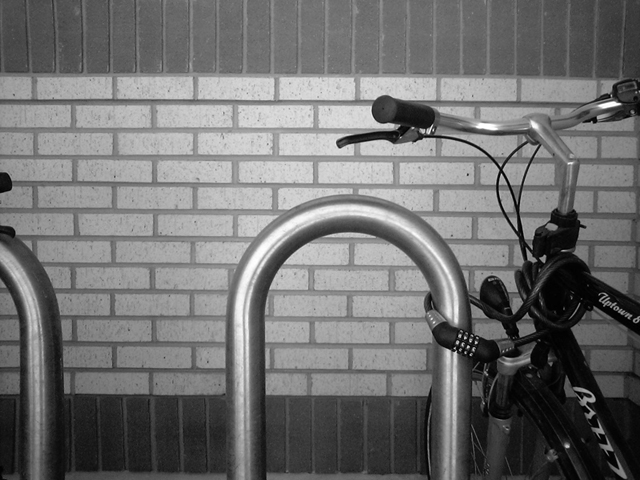
\includegraphics[width=\columnwidth]{img/bike_gray.jpg}
    \caption{Imagen en escala de grises de entrada}
    \label{fig:bike_gray}
  \end{subfigure}
  \hfill
  \begin{subfigure}{0.45\columnwidth}
      \centering
      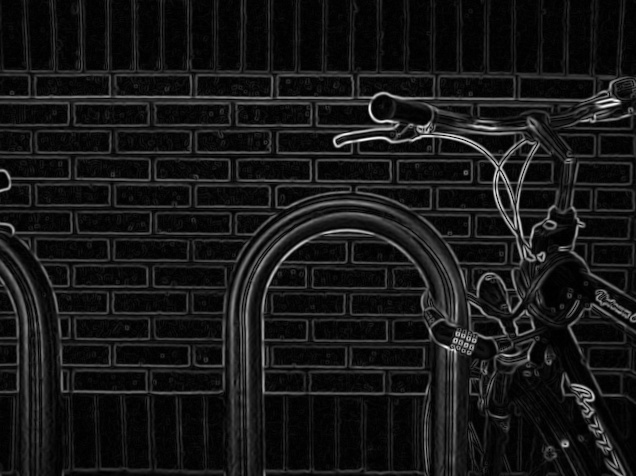
\includegraphics[width=\columnwidth]{img/bike_sobel.jpg}
      \caption{Salida del m\'odulo de procesamiento de video}
      \label{fig:bike_sobel}
  \end{subfigure}
  \hfill
    \caption{Ejemplo del procesamiento de video propuesto}
    \label{fig:processing_unit_example}
\end{figure}

El sistema adem\'as tendra los siguientes requerimientos:

\begin{itemize}
  \item \textbf{Cuadros procesados por segundo}: $60\ Hz$
  \item \textbf{Tama\~no de imagen}: $640\times480$ (est\'andar VGA)
  \item \textbf{Transmisi\'on}: Real-time (latencia m\'axima: $10\ ms$)
  \item \textbf{Presupuesto}: $< \$ 1000$
\end{itemize}


\section{Dise\~no}
\label{sec:design}

Basado en los requerimientos de la secci\'on \ref{sec:req} se deriva
el dise\~no para la aplicaci\'on presentado en la figura \ref{fig:block_diagram}.

\begin{figure}
  \centering

 \resizebox{\columnwidth}{!}{% 
  
    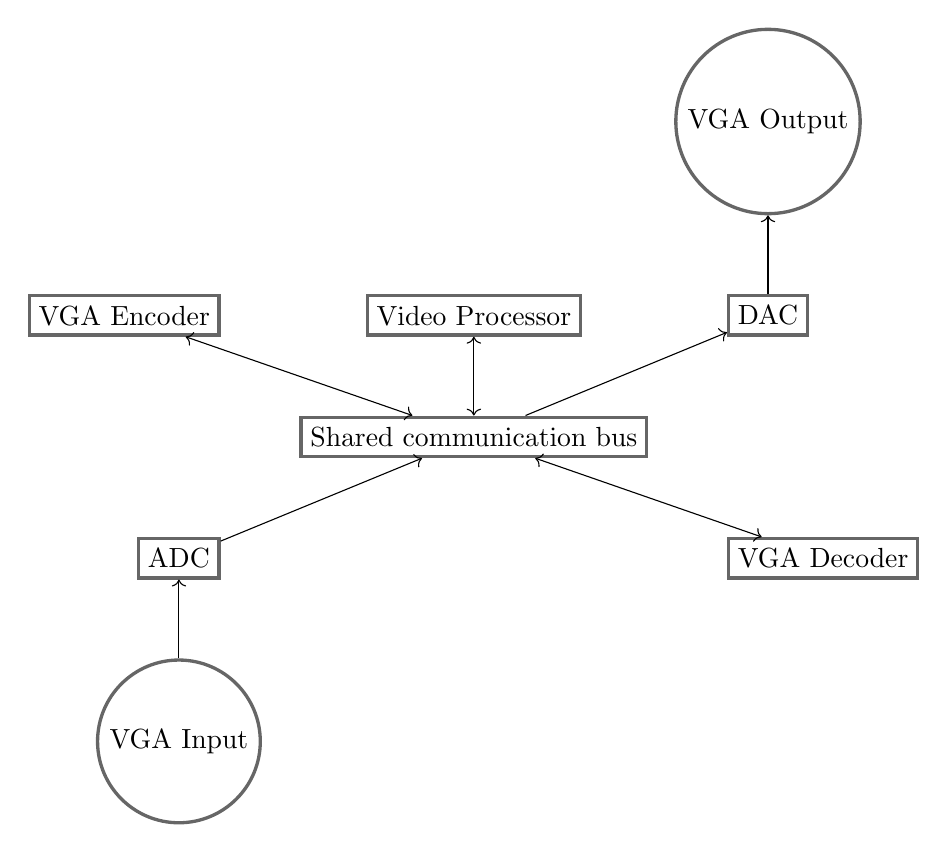
\begin{tikzpicture}[       ,
        roundnode/.style={circle, draw=black!60, very thick, minimum size=7mm},
        squarednode/.style={rectangle, draw=black!60, very thick, minimum size=5mm},
      ]
      % Nodes
    
      \node[squarednode] (bus) {Shared communication bus};
      
      \node[squarednode] (adc) [below left=of bus] {ADC};
      \node[squarednode] (vga_decoder) [below right=of bus] {VGA Decoder};
      \node[squarednode] (video_processor) [above=of bus] {Video Processor};
      \node[squarednode] (vga_encoder) [above left=of bus] {VGA Encoder};
      \node[squarednode] (dac) [above right=of bus] {DAC};
      
      \node[roundnode] (vga_input) [below=of adc] {VGA Input};
      \node[roundnode] (vga_output) [above=of dac] {VGA Output};    

      % Lines
      \draw[->] (vga_input) -- (adc);
      \draw[->] (adc) -- (bus);
      \draw[<->] (vga_encoder) -- (bus);
      \draw[<->] (video_processor) -- (bus);
      \draw[<-] (dac) -- (bus);
      \draw[<->] (vga_decoder) -- (bus);
      \draw[->] (dac) -- (vga_output);
    \end{tikzpicture}

}
    
  \caption{Diagrama de bloques de la soluci\'on}
  \label{fig:block_diagram}
\end{figure}

\section{Particionamiento de HW/SW}
\label{sec:partitioning}

El particionamiento ser\'a realizado de una manera funcional, es decir
se iniciara con las distintas funcionalidades a implementar y luego se
decidir\'a seg\'un la funcionalidad y los
requerimientos establecidos para decidir si el m\'odulo ser\'a
implementado en hardware o en software.

Tanto el m\'odulo de \emph{ADC} (Convertidor anal\'ogico a digital por
sus siglas en ingl\'es) como el m\'odulo de \emph{DAC} (Convertidor
digital a anal\'ogico por sus siglas en ingl\'es) son m\'odulos de
señal mixta por lo que deber\'an de ser implementados en hardware.

Para el modelado de los otros tres m\'odulos, este se realizar\'a de
la siguiente manera:

\begin{itemize}
    \item \textbf{Decodificador VGA}: Modelado \emph{Loosely Timed} (LT)
    \item \textbf{Procesador de imagen}: Modelado \emph{Programmer's view} (PV)
    \item \textbf{Codificador VGA}: Modelado \emph{Approximately Timed} (AT)
\end{itemize}

Ambos m\'odulos de codificaci\'on y decodificaci\'on son altamente 
dependientes en su temporizaci\'on para codificar y decodificar los datos
provenientes de la entrada VGA y devolverlos hacia otro m\'odulo de VGA con 
la temporizaci\'on correcta. Es por esto que estos m\'odulos ser\'an
implementados en hardware.

Por otro lado, el procesador de imagen ser\'a implementado en software,
debido a que este es m\'as apto para poder representar algoritmos
complejos con una alta precisi\'on. Adem\'as, estos son capaces de ser
modificados con una alta facilidad para extender sus capacidades, 
ya que los elementos de software son reconfigurables.

Debido a que el procesamiento de video ser\'a realizado en software, 
requerir\'a de un m\'odulo de memoria para almacenar la imagen antes 
y despu\'es del procesamiento. Esta memoria servir\'a, adem\'as como puente
entre los m\'odulos de decodificaci\'on, procesamiento y codificaci\'on, por
lo que se requiere de un bus que permita interconectar estos m\'odulos.

Aparte de una memoria, se requiere un procesador que permita ejecutar los
algoritmos de procesamiento de imagen propuestos para el 
\emph{video processor}. Para este caso, se preferir\'a un procesador 
vectorial, debido al manejo de memoria que se requiere para lograr mantener
el requerimiento de \emph{real-time} para la transmisi\'on. Un ejemplo de 
procesador a utilizar es un GPU (Unidad de procesamiento gr\'afico por sus
siglas en ingl\'es).

Adem\'as, se seleccion\'o la partici\'on mencionada porque se tiene la intenci\'on
de poder modificar el procesamiento una vez que el sistema est\'e implementado. 
Esto para tener la posibilidad de implementar cualquier otro algoritmo y que se 
cuente con el tiempo necesario de procesamiento sin afectar el rendimiento 
del sistema. Es decir, se est\'a dejando abierta la posibilidad de tardar 
m\'as en el procesamiento.

%\section{Conclusiones y Recomendaciones}

%------------------------------ CONCLUSIONS -----------------------------------%
Se presentaron los requerimientos para un sistema de adquisici\'on y procesamiento
de video que sigue el est\'andar VGA que opera a 60 cuadros por segundo y con una
latencia m\'axima de 10 ms.

El sistema propuesto procesar\'a la se\~nal adquirida cambi\'andola a escala de
grises y con un resaltamiento de bordes.

El sistema se dividir\'a en seis m\'odulos: ADC, decodificador, procesador, memoria,
codificador y DAC. De los cuales, el ADC y el DAC son de se\~nal mixta.

Los m\'odulos "Decodificador", "Procesador" y "Codificador", ser\'an modelados con los 
modelos de abstracci\'on \textit{loosely timed}, \textit{Programmer's view} y 
\text{Approximately Timed} respectivamente.

Respecto a la partici\'on Hardware/Software, los m\'odulos de codificador y 
decodificador ser\'an implementados por hardware, mientras que el procesador lo 
ser\'a por software.

%---------------------------- REFERENCES --------------------------------------%
%\newpage
% references section
\bibliography{hld}
\bibliographystyle{IEEEtran} 

% that's all folks
\end{document}
